\documentclass[10pt]{article}

%%notre fichier de configuration perso
\usepackage{rapport_configuration}


\usepackage[smartEllipses]{markdown}
\usepackage{pdfpages}
\usepackage{float}

\let\origfigure=\figure
\let\endorigfigure=\endfigure
\renewenvironment{figure}[1][]{%
  \origfigure[H]
}{%
  \endorigfigure
}

\title{%
DU CCIE
\\
{\normalsize Projet mathématiques et informatiques}
\\
Application Tournoi}
\author{    Thoma Lessage\\
            Pascal Padilla\\
            Raphaël Sellam
    }
\date{\today}



\begin{document}



%%% Titre coloré
\pagecolor{orangeamu!25}
\maketitle\thispagestyle{empty}





%%% Sommaire coloré
\newpage\pagecolor{orangeamu!10}
\tableofcontents


%%% couleur neutre


% \newpage
% \nopagecolor


\newpage


Dans le cadre du Diplôme Universitaire (DU) Compétences Complémentaires en Informatiques pour l'Enseignement (CCIE), les étudiants doivent participer à un projet math-info.

Nous avons décidé de créer une application multi plateforme : Tournoi. Nous exploitons pour cela le logiciel \href{https://godotengine.org/}{GODOT}.

Notre application est disponible pour différentes machines : Linux, Android, Windows, Windows universal, iOS et HTML5.





\subsubsection*{Site du projet}


Tout au long du projet, nous avons travaillé avec notre instance de Redmine : 
\url{https://pp.irem.univ-mrs.fr/projects/application-tournoi}




\subsubsection*{À propos de ce rapport}

Ce rapport est généré en \LaTeX à partir des \href{https://pp.irem.univ-mrs.fr/projects/application-tournoi/wiki/Wiki}{pages de notre wiki}.
\\
C'est pour cela que parfois la mise en page peut parfois paraître \textit{grotesque}\footnote{Avec des sauts de page un peu partout\ldots}.




\subsection*{Bonne lecture,}

~ \hfill
Thomas Lessage
\hfill 
Pascal Padilla
\hfill
Raphaël Sellam
\hfill ~





\newpage
\newpage\pagecolor{greenamu!15}
\markdownInput{Version_stable.txt.md}
\newpage


\newpage
\nopagecolor
\part{Présentation du projet et rendu}
\topskip0pt
\vspace*{\fill}
    \begin{center}
        
\includegraphics[width=0.5\linewidth]{Presentation_Tux_soldier.jpg}
    \end{center}
\vspace*{\fill}

\newpage

\markdownInput{Appel_a_projet.txt.md}
\newpage
\markdownInput{Road_map.txt.md}




\newpage
\part{Gestion du projet et outils}
\topskip0pt
\vspace*{\fill}
    \begin{center}
        
\includegraphics[width=0.5\linewidth]{Outils_tux-161507_960_720.png}
    \end{center}
\vspace*{\fill}
\newpage

\markdownInput{Scrum.txt.md}
\newpage
\markdownInput{Godot.txt.md}
\newpage
\markdownInput{Depot_git.txt.md}
\newpage
\markdownInput{Tests_unitaires_avec_GUT.txt.md}
\newpage
\markdownInput{Generateur_automatique_de_doc.txt.md}



\newpage
\part{Documentation et références techniques}
\topskip0pt
\vspace*{\fill}
    \begin{center}
        
\includegraphics[width=0.5\linewidth]{Doc_tux-161406_960_720.png}
    \end{center}
\vspace*{\fill}
\newpage

La documentation de l'application est disponible en ligne\footnote{Et nettement mieux présentée que dans ce rapport. L'import de texte au format markdown génère quelques ratés, notamment sur la gestions du caractère \_.} : \url{https://github.com/Pskalou/tournoi/tree/master/source/doc}.

\markdownInput{../source/doc/Game_generator.md}
\newpage
\markdownInput{../source/doc/Score_manager.md}
\newpage
\markdownInput{../source/doc/Duel_button.md}
\newpage
\markdownInput{../source/doc/Round_buttons.md}




\newpage
\part{Annexe}
\topskip0pt
\vspace*{\fill}
    \begin{center}
        
\includegraphics[width=0.5\linewidth]{Annexe_Tux_Spallanzani.png}
    \end{center}
\vspace*{\fill}
\newpage


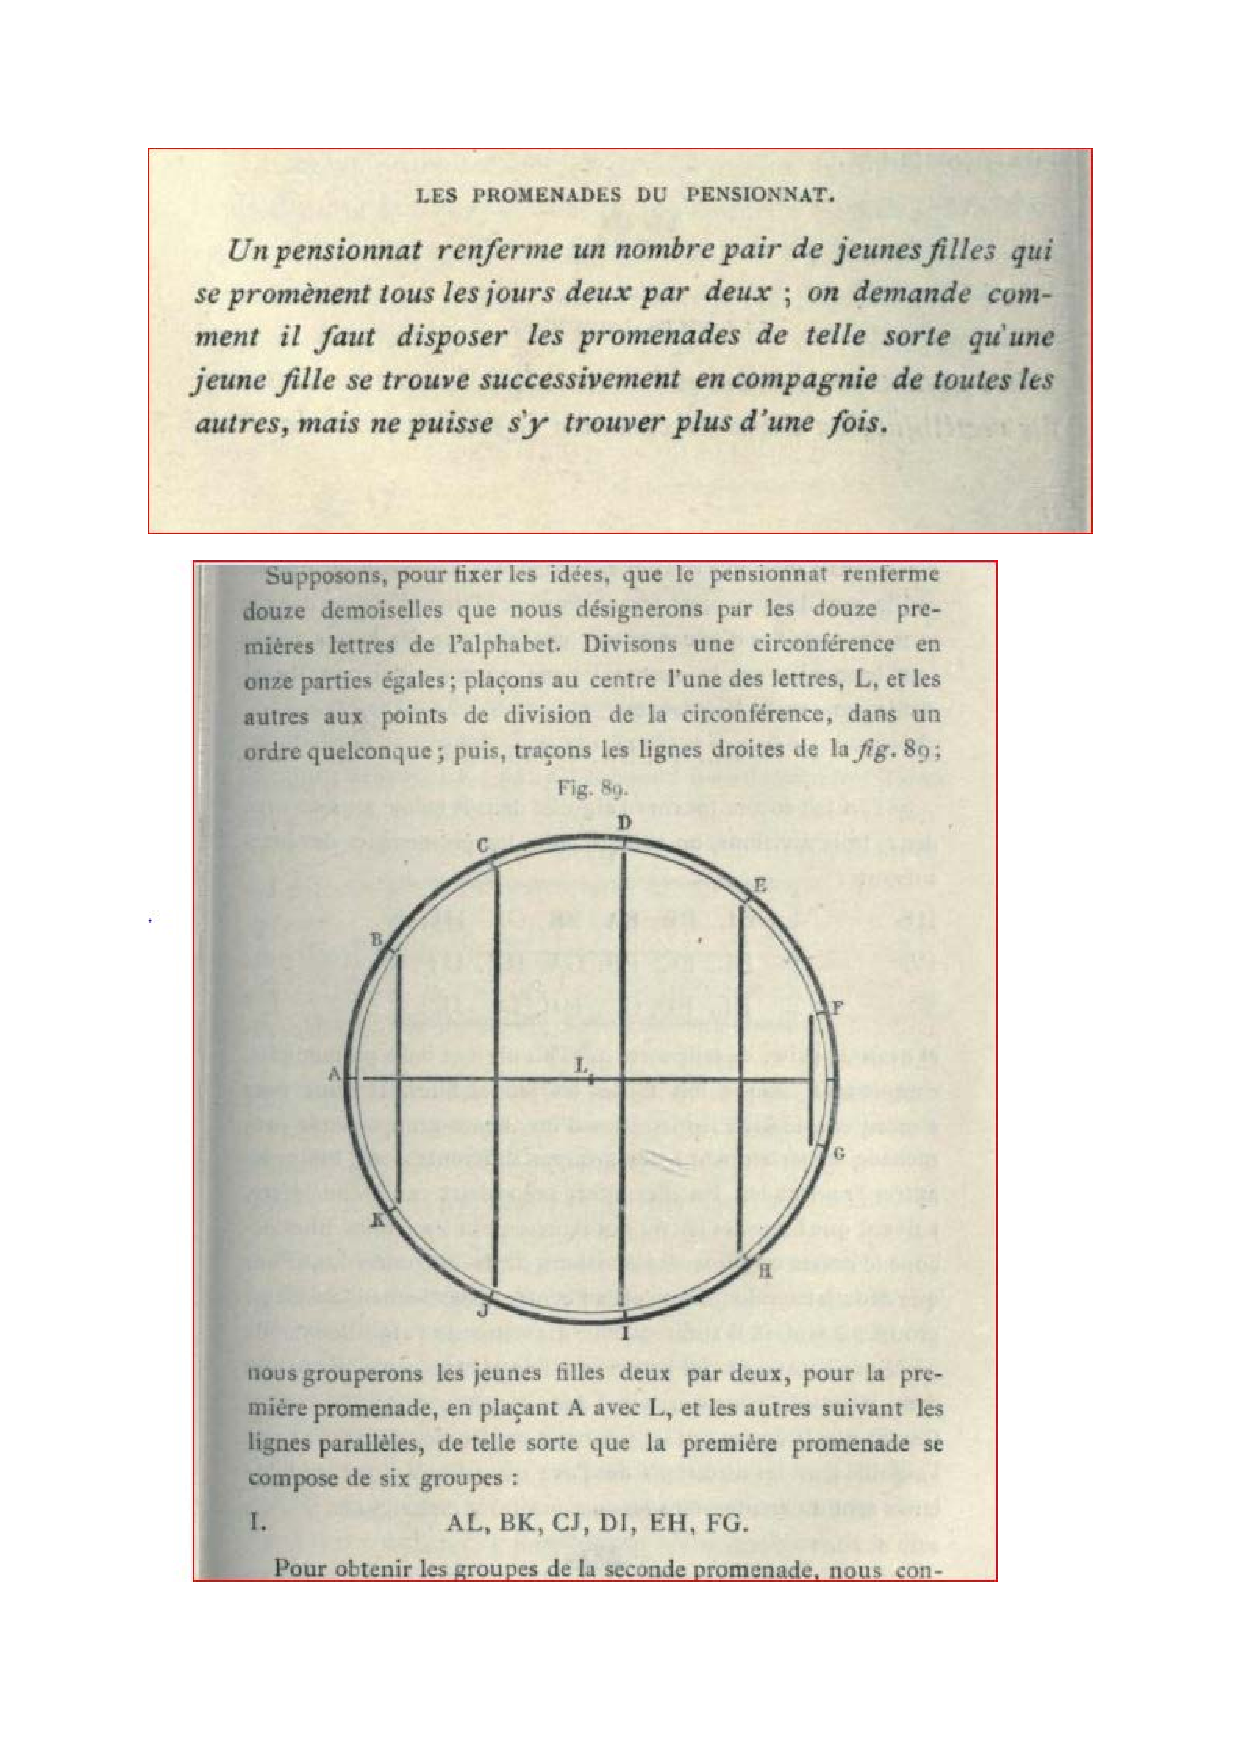
\includepdf[scale=.8, page=1, pagecommand=\section{Une approche mathématique}]{Projet_Tournois.pdf}
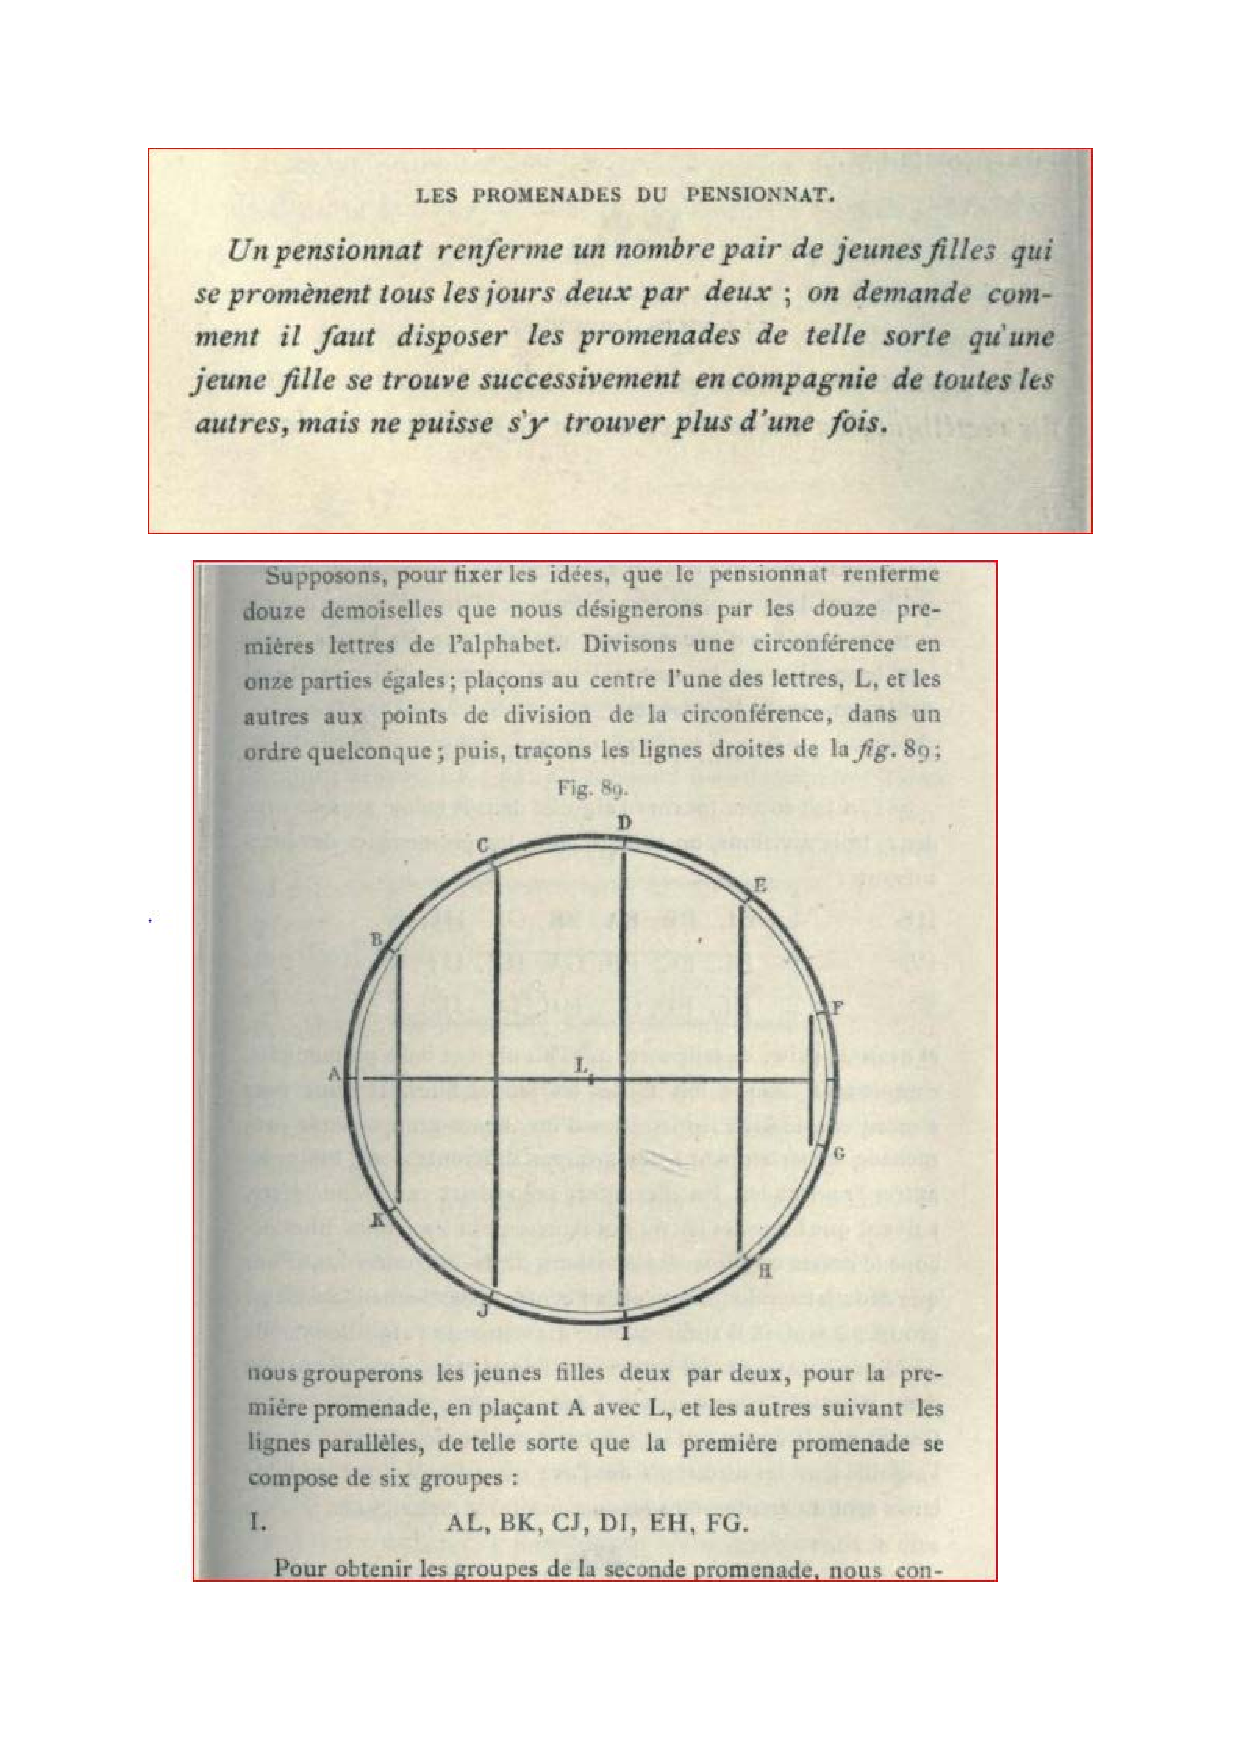
\includepdf[scale=.9, page=2-4]{Projet_Tournois.pdf}
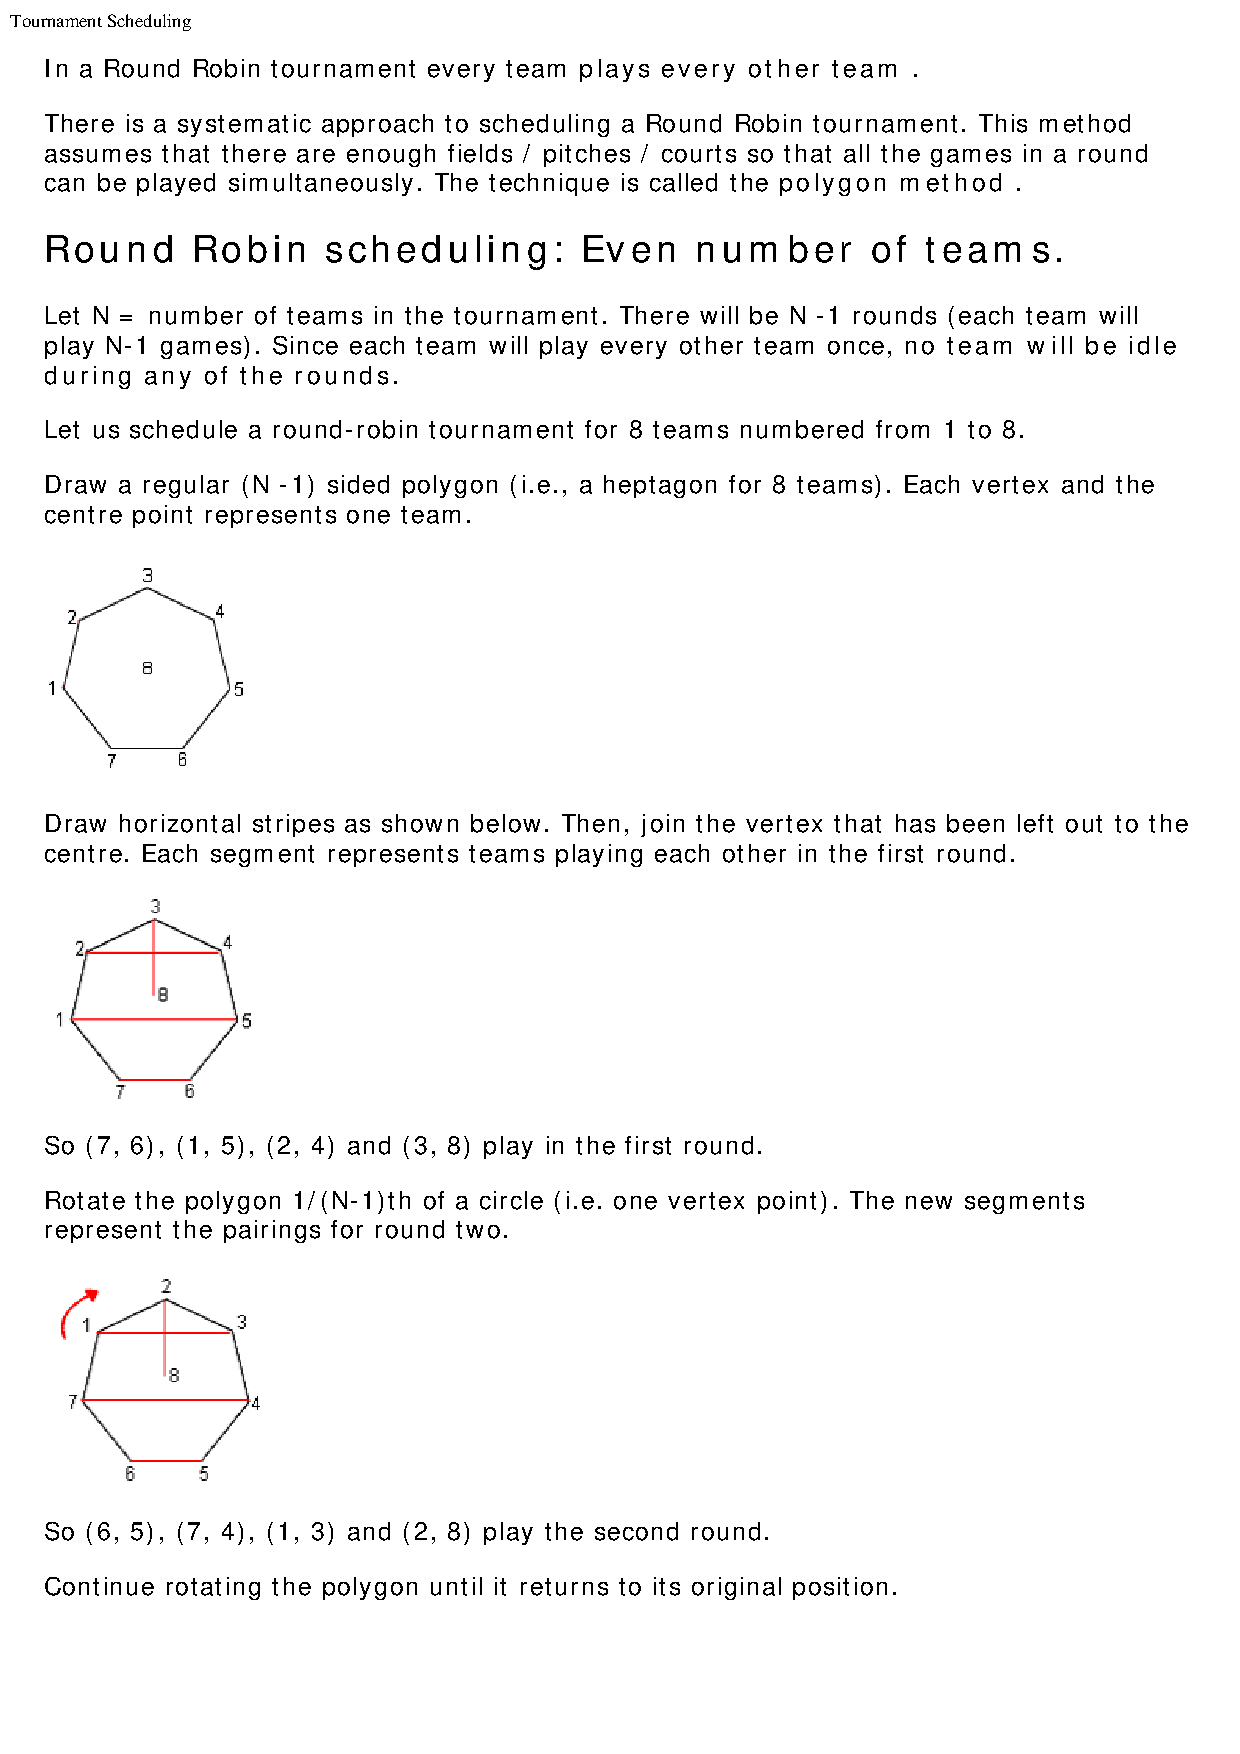
\includepdf[scale=.9, page=2-4]{Projet_Tournois_Bis.pdf}

\newpage
\markdownInput{Sprint_et_visioconf.txt.md}
% \newpage
% \markdownInput{Version_beta.txt.md}
% \newpage
% \markdownInput{Version_alpha.txt.md}

\end{document}